% VUT FIT MITAI
% MSZ 2021/2022
% Author: Vladimir Dusek
% Login: xdusek27

%%%%%%%%%%%%%%%%%%%%%%%%%%%%%%%%%%%%%%%%%%%%%%%%%%%%%%%%%%%%%%%%%%%%%%%%%%%%%%%%

% Path to figures
\graphicspath{{upa/prostorove_db_indexace/figures}}

%%%%%%%%%%%%%%%%%%%%%%%%%%%%%%%%%%%%%%%%%%%%%%%%%%%%%%%%%%%%%%%%%%%%%%%%%%%%%%%%

\chapter{UPA~--~Indexace (nejen) v prostorových DB (kD-Tree a Grid File (a jejich varianty), R-Tree).}

%%%%%%%%%%%%%%%%%%%%%%%%%%%%%%%%%%%%%%%%%%%%%%%%%%%%%%%%%%%%%%%%%%%%%%%%%%%%%%%%

\section{Zdroje}

\begin{compactitem}
    \item \path{PDB-Spatial-CZ.pdf}
    \item \path{03-spatial_databases.pdf}
    \item \path{szz-kastak.pdf}
    \item \path{szz-discord-bazi.pdf}
\end{compactitem}

%%%%%%%%%%%%%%%%%%%%%%%%%%%%%%%%%%%%%%%%%%%%%%%%%%%%%%%%%%%%%%%%%%%%%%%%%%%%%%%%

\section{Úvod a kontext}

\begin{compactitem}
    \item Ve vícedimenzionálním prostoru nelze z reprezentace hodnot jednoznačně určit uspořádání -- předchůdce a následníka. Nelze tedy použít obecně užívané indexační algoritmy pro 1D.

    \item Řešení v podobě mapování do 1D nám většinou nestačí, proto se v prostorových databázích využívají specializované indexační algoritmy.
\end{compactitem}

%%%%%%%%%%%%%%%%%%%%%%%%%%%%%%%%%%%%%%%%%%%%%%%%%%%%%%%%%%%%%%%%%%%%%%%%%%%%%%%%

\section{Mapování do 1D}

\begin{compactitem}
    \item Nejjednodušší řešení je namapovat data do jednorozměrného prostoru.
    \item Touto transformací však zcela jistě ztratíme sousednost.
    \item Krom toho, taková transformace nemusí být vůbec realizovatelná. A pokud ano, tak výsledek dotazů nemusí být transformovatelný zpět, takže lze výsledek jen těžko interpretovat.
\end{compactitem}

%%%%%%%%%%%%%%%%%%%%%%%%%%%%%%%%%%%%%%%%%%%%%%%%%%%%%%%%%%%%%%%%%%%%%%%%%%%%%%%%

\section{Indexace bodů}

\begin{compactitem}
    \item Pro indexaci bodů využíváme 2 přístupy: stromy dělící prostor a hashování.
\end{compactitem}

\subsection{Stromy dělící prostor}

\subsubsection{k-D Tree}

\begin{compactitem}
    \item k-D Tree je datová struktura (binární strom) dělící prostor hyperplochami na nejvyšší možné úrovni, a to vždy na dvě části. \begin{compactitem}
        \item Hyperplocha v rovině je přímka.
        \item Dělící hyperplocha musí být rovnoběžná s osovým (souřadným) systémem.
    \end{compactitem}

    \item Myšlenka: vytvoříme uspořádání na množině bodů v prostoru (podobně jako ho máme přirozeně na množině čísel) a díky tomu, budeme moct uspořádat body do stromu.

    \item Při dělení, musí ve výsledných plochách být obsažen vždy aspoň jeden bod, který pak už není součástí jakékoli jiné hyperplochy.

    \item Vkládání a vyhledávání je bez problému, avšak při mazání je potřeba znovuustavit celý strom, algoritmus je tak vhodný pro statická data.

    \item Pořadí vkládání bodů výrazně ovlivňuje vyváženost výsledného stromu.
\end{compactitem}

\begin{figure}[H]
    \centering
    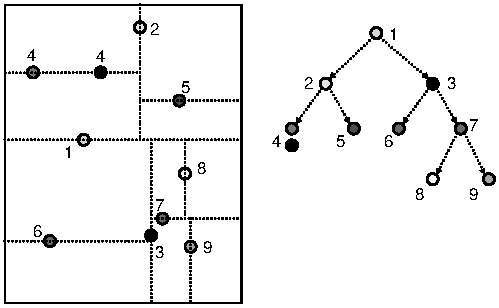
\includegraphics[width=0.75\linewidth]{kd_tree.pdf}
    \caption{k-D tree.}
\end{figure}

\subsubsection{Adaptivní k-D Tree}

\begin{compactitem}
    \item Snaží se eliminovat problémy spojené s pořadím vkládání bodů.
    \item Shodný s k-D Tree, až na to, že dělící hyperplochy \begin{compactitem}
        \item už nemusí obsahovat nějaký bod, stačí, že dělí prostor;
        \item jsou vybírány tak, aby výsledný prostor obsahoval přibližně stejný počet bodů.
    \end{compactitem}
    \item Ze změn vyplývá, že data jsou uložena až v listových uzlech.
    \item Algoritmus je stále vhodný pro statická data.
\end{compactitem}

\begin{figure}[H]
    \centering
    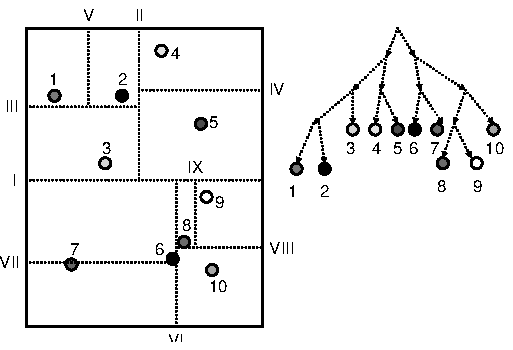
\includegraphics[width=0.75\linewidth]{adaptivni_kd_tree.pdf}
    \caption{Adaptivní k-D Tree.}
\end{figure}

\subsubsection{BSP (\textit{binary space partitioning}) Tree}

\begin{compactitem}
    \item Stejný jako Adaptivní k-D Tree až na to, že dělící hyperplochy nemusí být rovnoběžné s osovým (souřadným) systémem.
    \item Prostor se dělí do doby, než počet bodů v ploše neklesne pod určitou hodnotu (na obrázku 2).
    \item Má vyšší nároky na paměť než k-D Tree, u kterého šlo díky pravidelnému střídání dělení ignorovat jednu souřadnici hyperplochy.
\end{compactitem}

\begin{figure}[H]
    \centering
    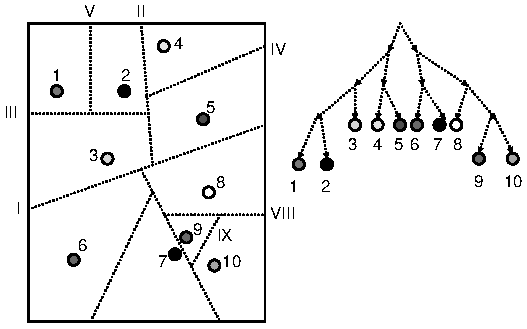
\includegraphics[width=0.75\linewidth]{bsp_tree.pdf}
    \caption{BSP Tree.}
\end{figure}

\subsubsection{Quad Tree}

\begin{compactitem}
    \item Stejný jako k-D Tree až na to, že prostor se dělí na čtvrtiny (dvě dělící hyperplochy na bod).
    \item Prostor se dělí do doby, než počet bodů v ploše neklesne pod určitou hodnotu (na obrázku 2).
    \item Některé prostory neobsahují žádný bod.
\end{compactitem}

\begin{figure}[H]
    \centering
    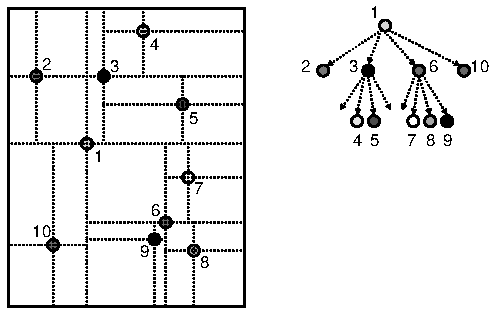
\includegraphics[width=0.75\linewidth]{quad_tree.pdf}
    \caption{Quad Tree.}
\end{figure}

\subsection{Hashování}

\subsubsection{Grid File}

\begin{compactitem}
    \item Sledovaný úsek prostoru je rozdělen $n$-rozměrnou mřížkou (ne nutně pravidelnou) na buňky. \begin{compactitem}
        \item Buňky obsahují různý počet bodů, klidně 0.
    \end{compactitem}

    \item Dále existuje adresář, který každou buňku přiřazuje k datové jednotce (\textit{bucket}). \begin{compactitem}
        \item Adresář je poměrně velký a spolu s mřížkou je vždy ukládán na disk.
    \end{compactitem}

    \item Při vkládání může dojít k přetečení (datová jednotka není schopna pojmout další údaj), které není lokální. \begin{compactitem}
        \item Je nutné vložit rozdělující hyperplochu a tak zvětšit adresář.
        \item Podobně se chová i mazání -- jelikož není lokální, tak odstranění hyperplochy je třeba prověřit. Pokud je dat málo, tak může zaniknout i datová jednotka (data buďto zanikla s ní, nebo jsou přesunuta do jiné datové jednotky).
    \end{compactitem}
\end{compactitem}

\begin{figure}[H]
    \centering
    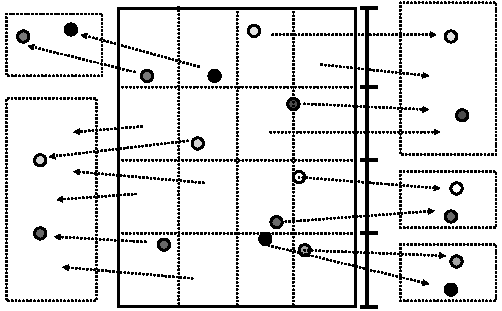
\includegraphics[width=0.75\linewidth]{grid_file.pdf}
    \caption{Grid File.}
\end{figure}

\subsubsection{Two-level Grid File}

\begin{compactitem}
    \item Je zavedena mřížka druhé úrovně. \begin{compactitem}
        \item První úroveň slouží pouze jako ukazatel do základní struktury Grid filu.
    \end{compactitem}

    \item V takovém systému jsou změny při vkládání či mazání často lokální, nicméně i tak není problematika přetečení úplně vyřešena.
\end{compactitem}

\begin{figure}[H]
    \centering
    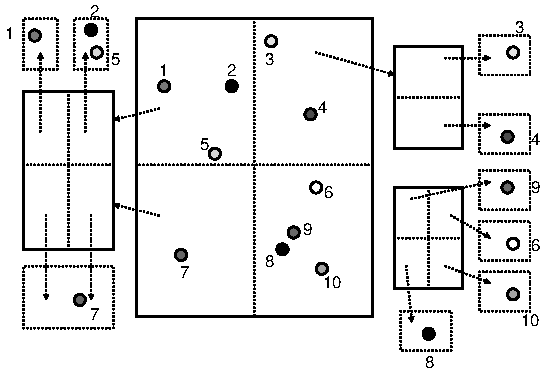
\includegraphics[width=0.75\linewidth]{grid_file_two_level.pdf}
    \caption{Two-level Grid File.}
\end{figure}

\subsubsection{Twin Grid File}

\begin{compactitem}
    \item Celá struktura se vyskytuje dvakrát. \begin{compactitem}
        \item Vztah však není hierarchický (vertikální), ale horizontální.
        \item I když je jedna ze struktur nadřazená, tak je jedno, která to bude.
    \end{compactitem}
    \item Cílem tohoto algoritmu je maximálně využít prostor pro indexovací strukturu. \begin{compactitem}
        \item Data se mezi obě části dělí prakticky rovnoměrně.
        \item Jedna struktura je však primární a druhá je sekundární, přetoková.
    \end{compactitem}
    \item Algoritmus má úplnou paralelizaci vyhledávání a částečnou pro vkládání.
\end{compactitem}

\begin{figure}[H]
    \centering
    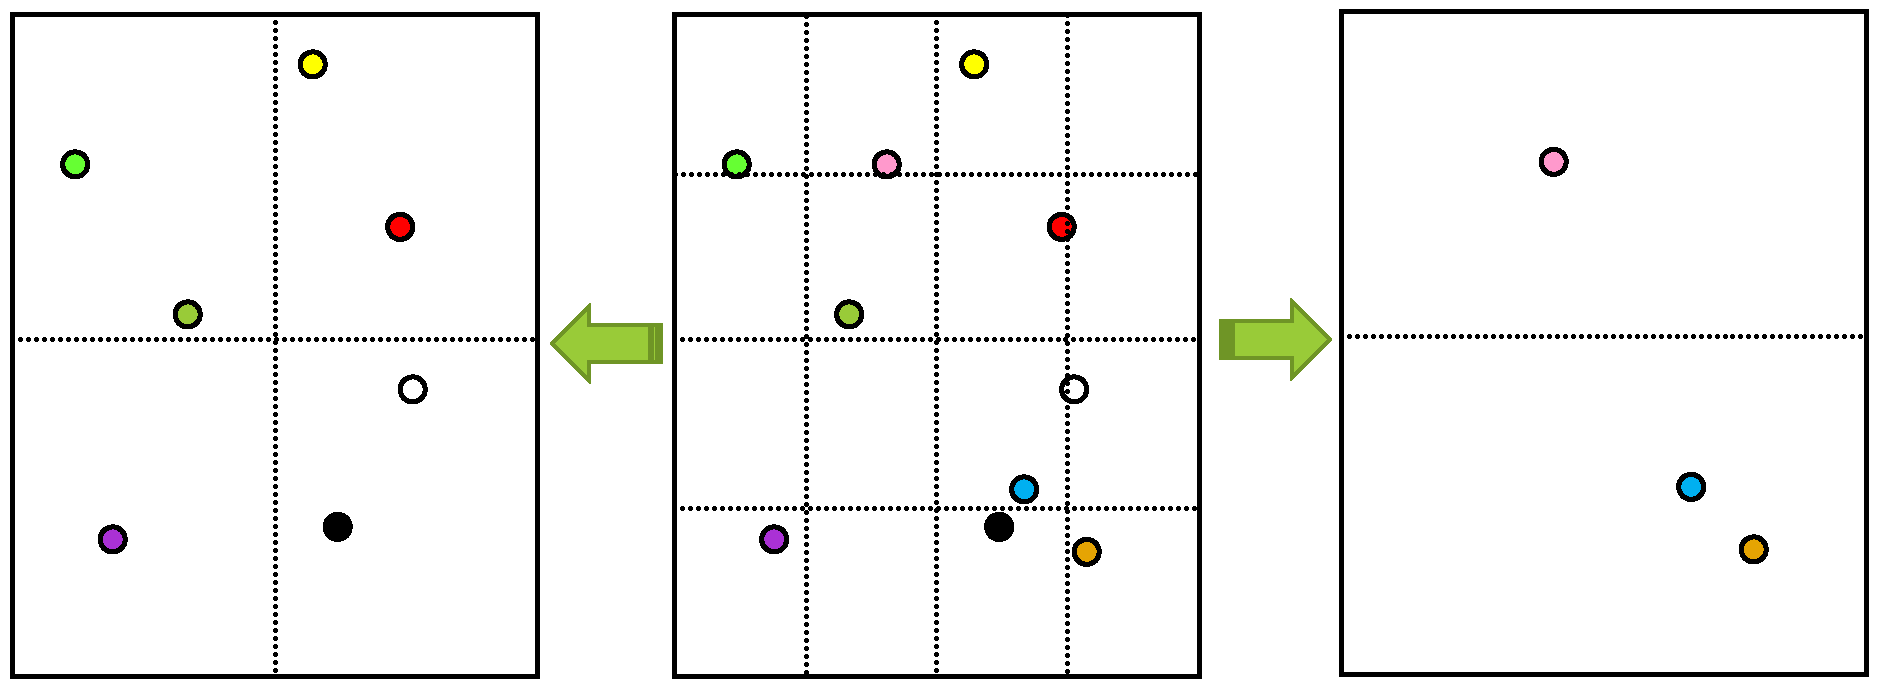
\includegraphics[width=0.9\linewidth]{grid_file_twin.pdf}
    \caption{Twin Grid File.}
\end{figure}

%%%%%%%%%%%%%%%%%%%%%%%%%%%%%%%%%%%%%%%%%%%%%%%%%%%%%%%%%%%%%%%%%%%%%%%%%%%%%%%%

\section{Indexace vícerozměrných objektů}

\begin{compactitem}
    \item Uložení bodů je sice primární, ale v obecné realitě s ním nelze vystačit, proto vznikly algoritmy pro indexaci vícerozměrných útvarů, které používají buďto překrývání (\textit{overlapping}) a nebo ořezávání (\textit{clipping}).
\end{compactitem}

\subsection{Překrývání -- R-Trees}

\begin{compactitem}
    \item Indexační struktury se překrývají, takže vzniká více vyhledávacích cest, implementačně se buňky překrývají svými hranicemi.

    \item V praxi tak dochází k tomu, že algoritmus je stejný, jen počet prohledávacích cest se zvětšuje, protože dopředu není jasné, ve které buňce je nakonec objekt uložen.
\end{compactitem}

\begin{figure}[H]
    \centering
    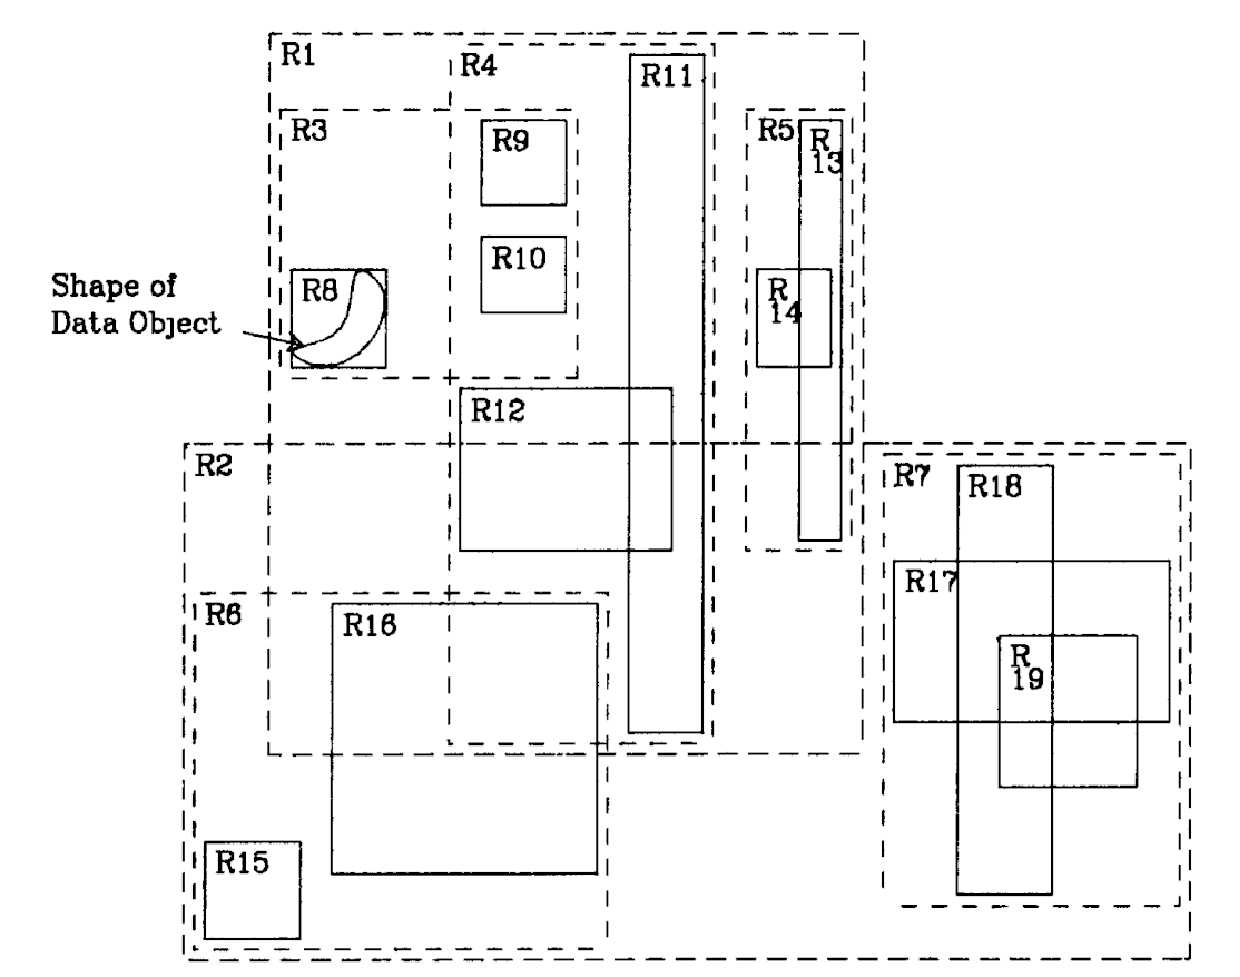
\includegraphics[width=0.85\linewidth]{r_tree_1.pdf}
    \caption{R-Tree příklad.}
\end{figure}

\begin{figure}[H]
    \centering
    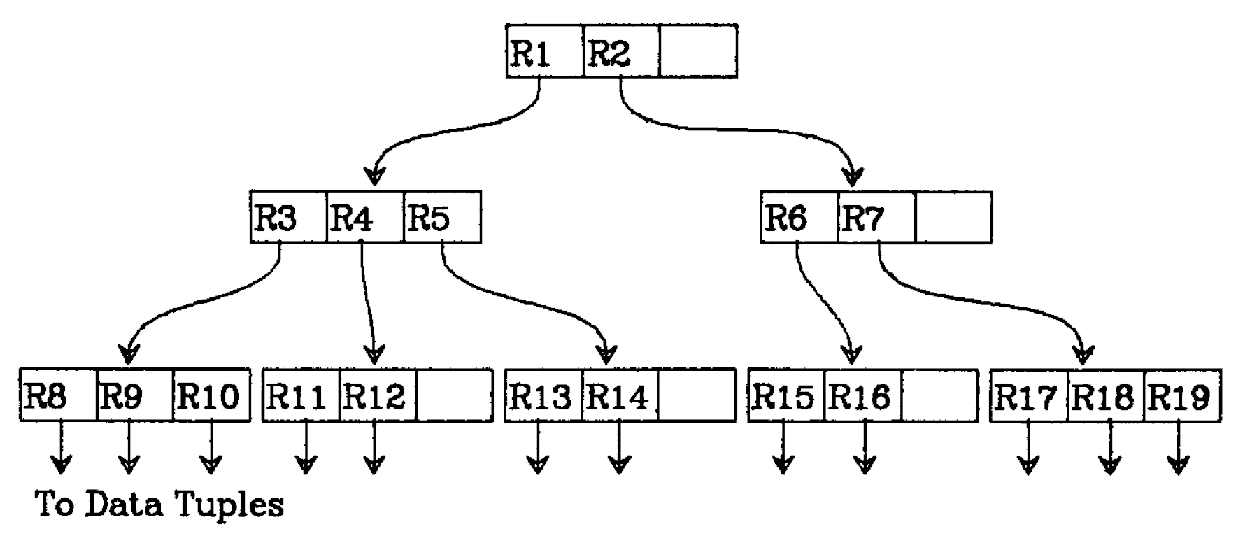
\includegraphics[width=0.85\linewidth]{r_tree_2.pdf}
    \caption{R-Tree příklad -- index.}
\end{figure}

\subsection{Ořezávání -- $\text{R}^+$-Trees}

\begin{compactitem}
    \item U metod založených na ořezávání není povoleno, aby se MBB (\textit{minimal bounding box}), buňky překrývaly.
    \item Jediným řešením je rozsekat objekty tak, aby sledovaly hranice dělicích MBB. Jeden objekt tak může být rozdělen na více.
    \item Při vyhledávání pak tedy nestačí vyhledat objekt, ale je třeba se vrátit k jeho původní, nedělené reprezentaci.
\end{compactitem}

\begin{figure}[H]
    \centering
    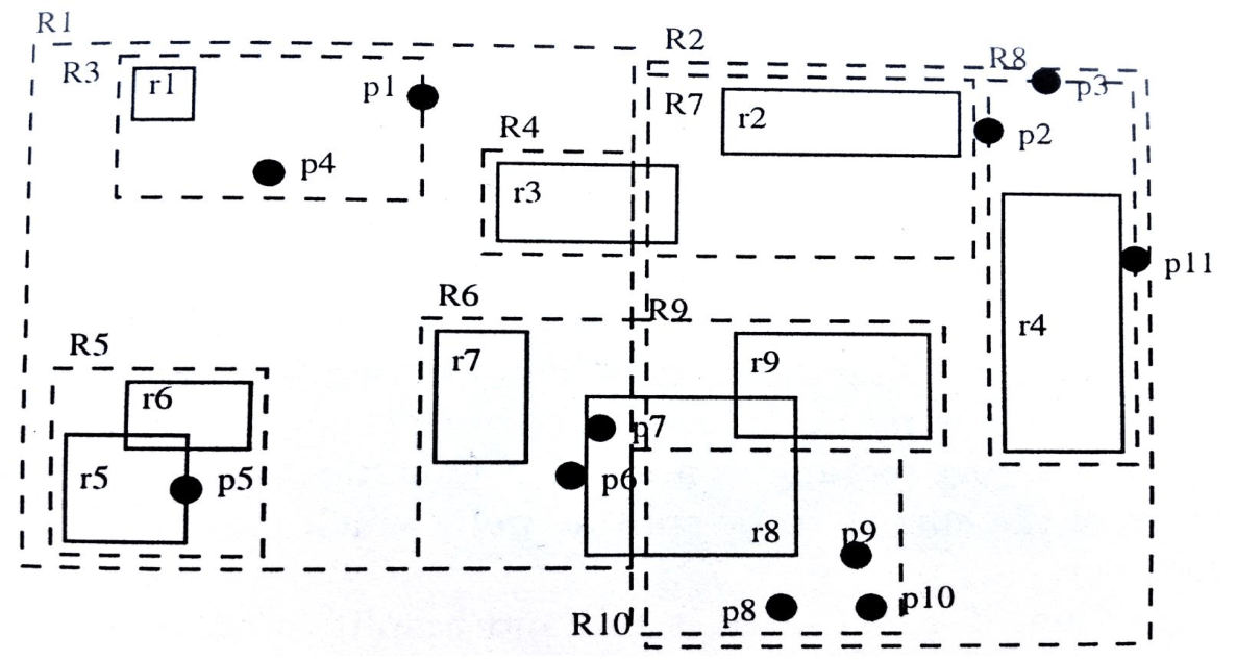
\includegraphics[width=0.85\linewidth]{r_tree_plus_1.pdf}
    \caption{$\text{R}^+$-Tree příklad.}
\end{figure}

\begin{figure}[H]
    \centering
    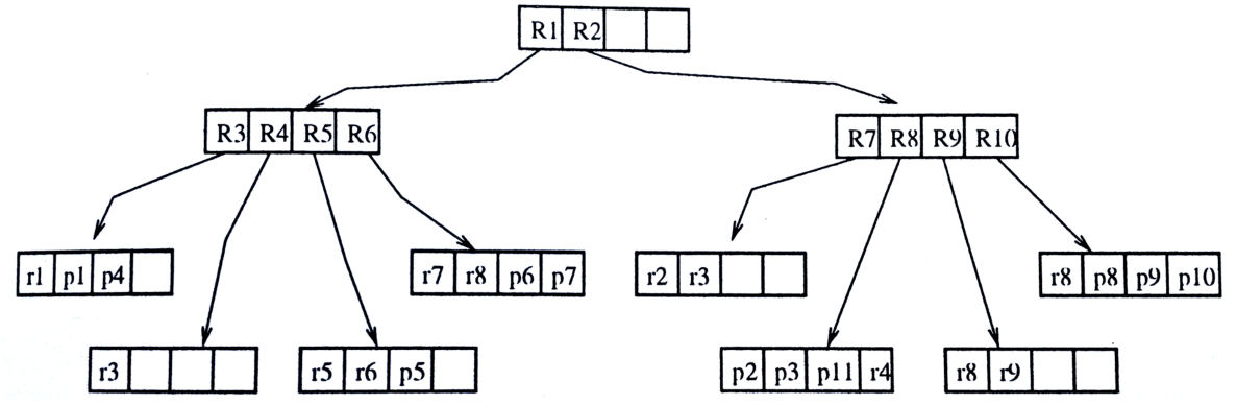
\includegraphics[width=1\linewidth]{r_tree_plus_2.pdf}
    \caption{$\text{R}^+$-Tree příklad -- index.}
\end{figure}
